\chapter{Desenvolvimento}
\label{cap:Desenvolvimento}
Nesse capítulo serão abordadas todas as etapas, tal como as técnicas utilizadas para atingir o objetivo de compor um dicionário de léxicos da língua portuguesa específico para detecção de discursos de ódio. Ao final também serão apresentados os resultados esperados com o desenvolvimento, estimando a eficiência e os avanços da pesquisa realizada. 

\section{Geração de \textit{corpus} para Detectar \textit{Haters}}
Como parte fundamental da pesquisa, será criado um dicionário com as palavras mais utilizadas pelos usuários denominados \textit{haters} que pregam discursos de ódio contra indivíduos nas redes sociais.Para a geração do \textit{corpus} desejado serão necessárias algumas etapas de desenvolvimento conforme Figura \ref{fig:fluxodesenvolvimento}. A seguir serão explicadas cada uma das etapas a serem realizadas para a obtenção do dicionário.

\begin{figure}[!h]
\centering 
\caption{Fluxo de atividades para obtenção de \textit{corpus} desejado}
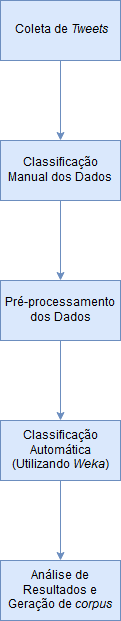
\includegraphics[scale=0.5]{imagens/fluxodesenvolvimento.png}
\legend{Fonte: O Autor}
\label{fig:fluxodesenvolvimento}
\end{figure}

\subsection{Coleta de \textit{Tweets}}
\label{subsec:coletatweets}
A rede social selecionada para a construção da base de dados será o \textit{Twitter}, rede social categorizada como \textit{microblogging} em que os usuários realizam atualizações constantes de conteúdo sendo ele textual, de figuras, vídeos, enquetes e etc. No contexto da rede social, as postagens dos usuários recebem o nome de \textit{tweet} e tem o limite de $280$ caracteres. 
Para realizar a coleta de dados primeiramente é necessário criar uma conta dentro da \textit{Twitter Developer Platform}\footnote{https://developer.twitter.com/}. Após cadastro a plataforma disponibilizará os \textit{tokens} que serão necessários para a construção do programa de leitura de \textit{tweets} (Figura \ref{fig:twitterdeveloperplatform}).

\begin{figure}[!h]
\centering 
\caption{Tela com \textit{Tokens} Utilizados na \textit{API} do \textit{Twitter}}
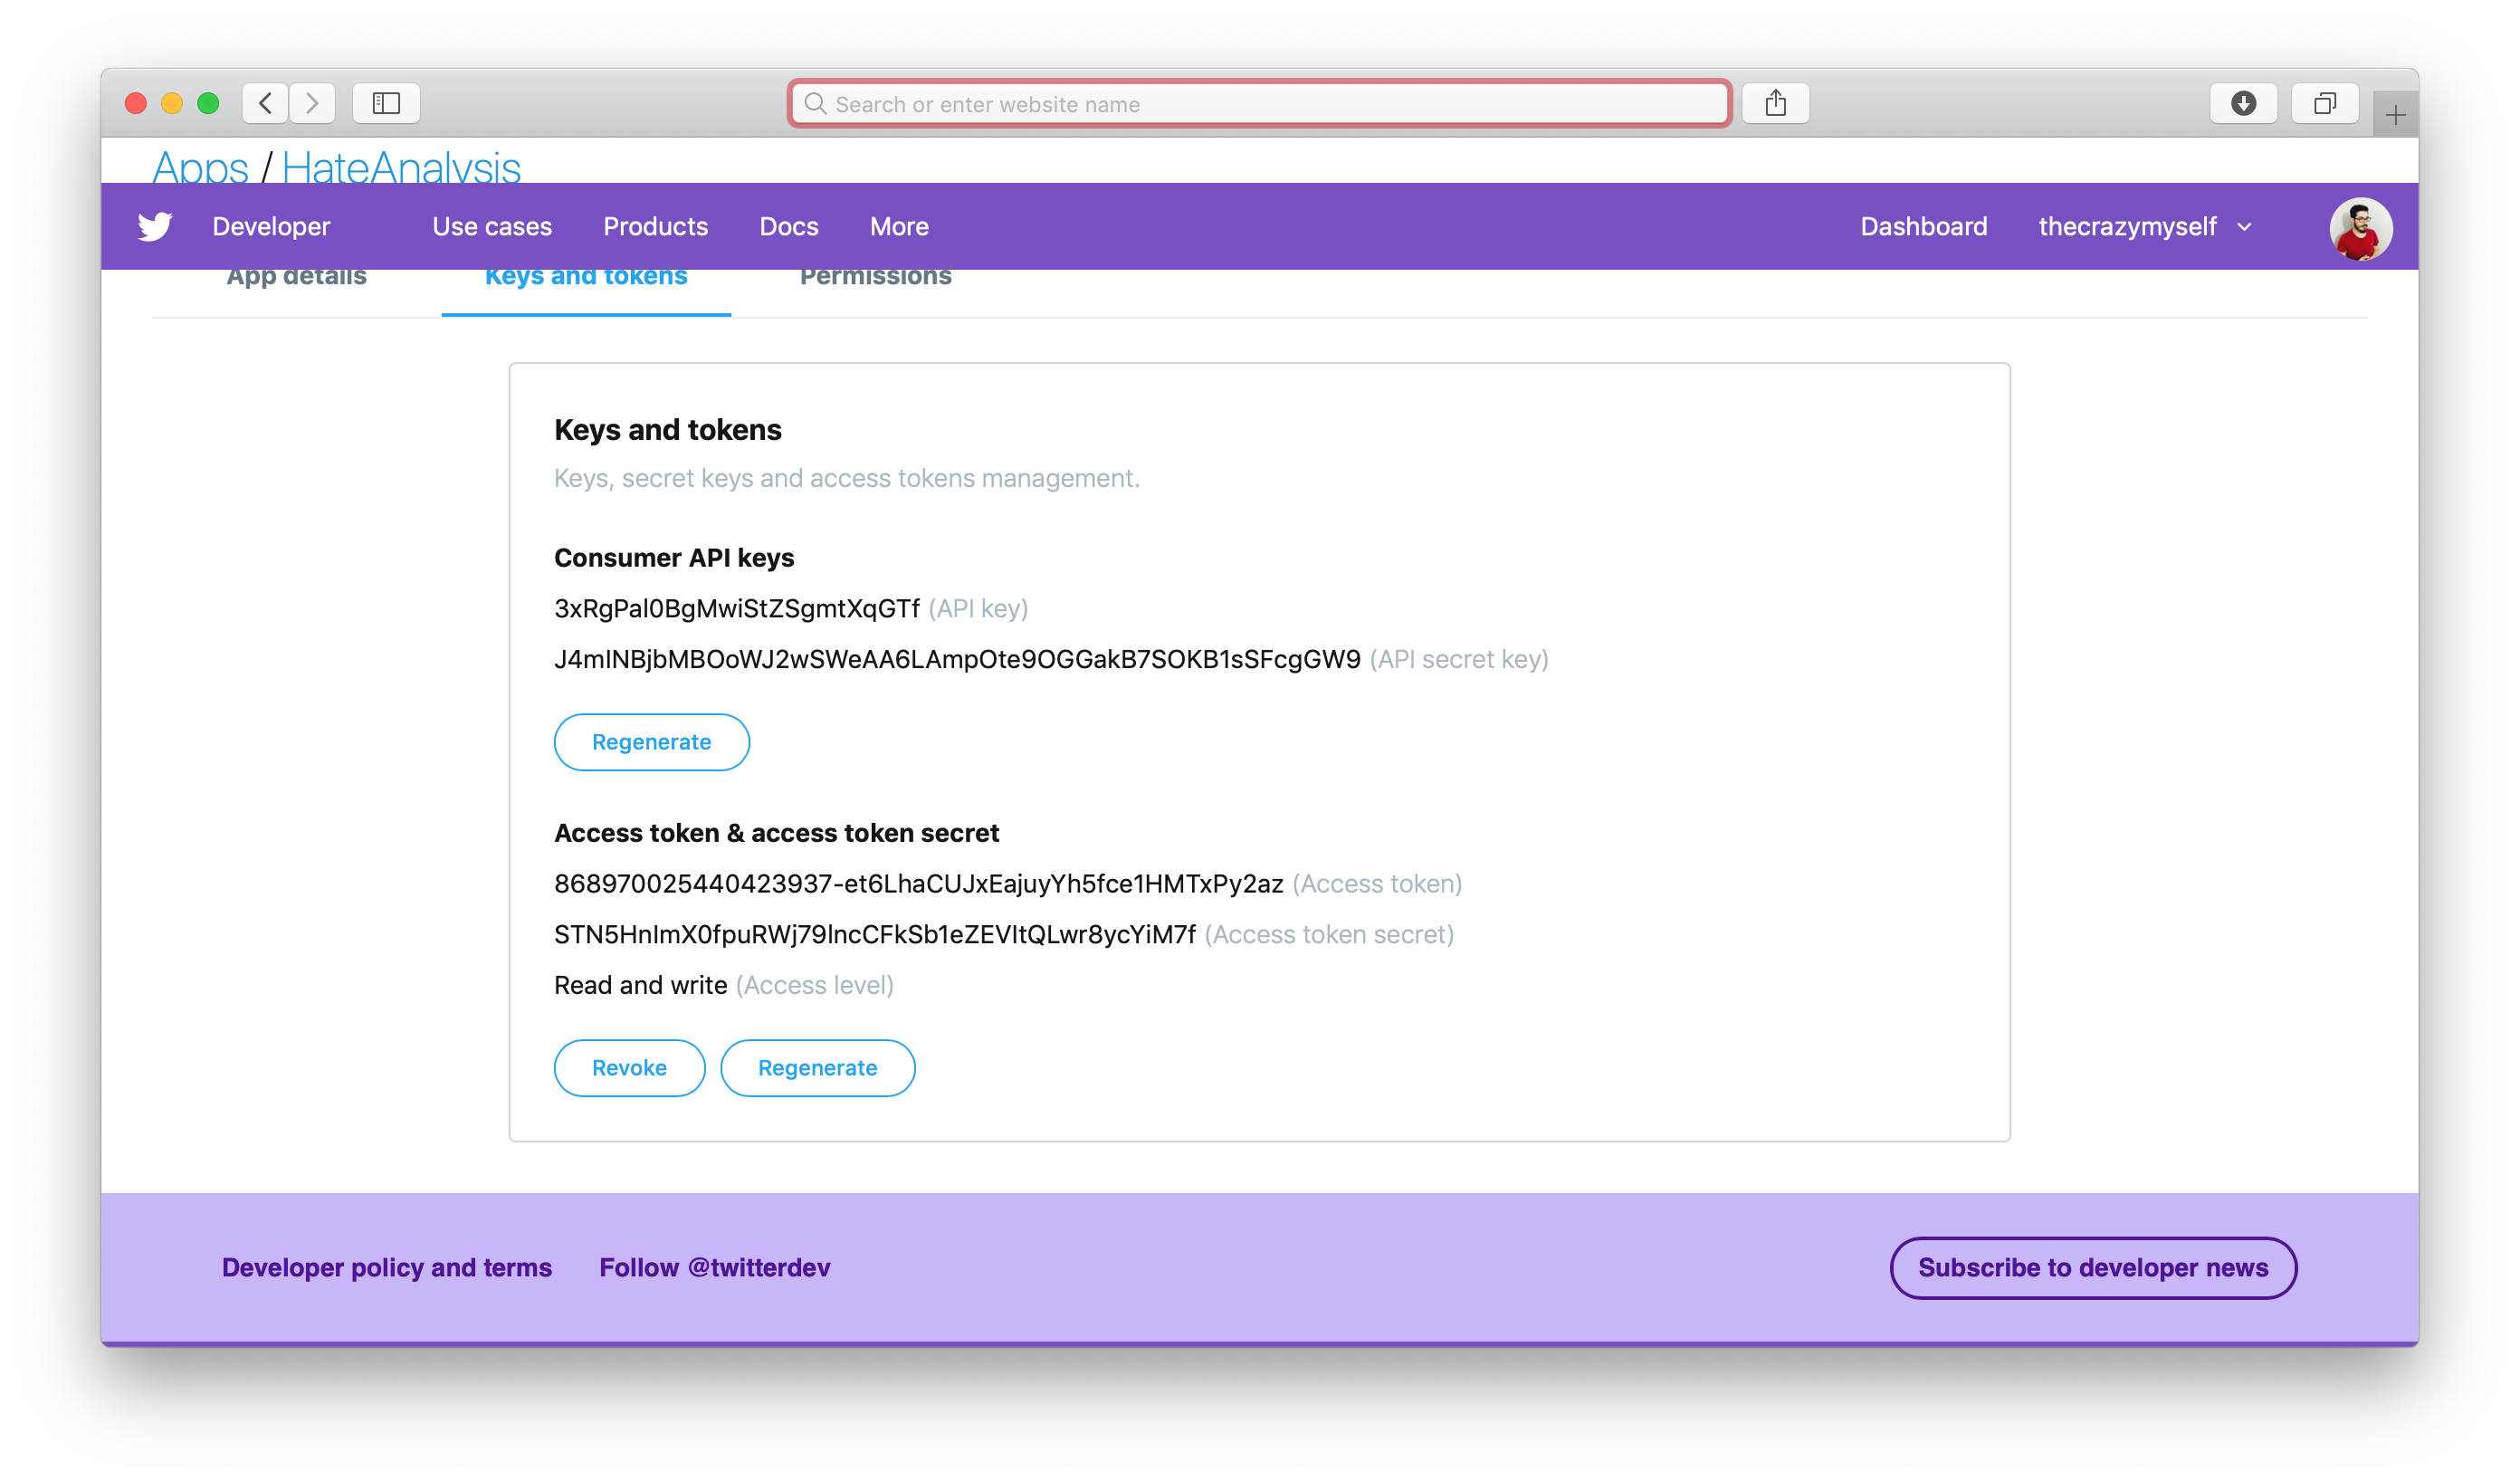
\includegraphics[scale=0.3]{imagens/twitterdeveloperplatform.png}
\legend{Fonte: Twitter Inc.}
\label{fig:twitterdeveloperplatform}
\end{figure}

A linguagem de programação a ser utilizada para a coleta dos dados será a \textit{Java}, linguagem orientada a objetos e multiplataforma mantida pela \textit{Oracle} que é de fácil implementação e bastante utilizada na comunidade \textit{open source} que mantém vários fóruns, \textit{frameworks} e \textit{APIs} constantemente atualizados pela comunidade. A \textit{API} que utilizada será a \textit{Twitter4J}, uma biblioteca não-oficial que permite o acesso aos dados do \textit{Twitter} utilizando a linguagem de programação \textit{Java}, a mesma que será utilizada para a coleta de dados, facilitando o aprendizado da ferramenta bem como a manutenção, se necessário. A \textit{Twitter4J} utiliza autenticação \textit{OAuth}, fazendo uso dos \textit{tokens} disponibilizados pelo \textit{Twitter Developer Platform} e não necessitando de autenticação com e-mail (ou nome de usuário, ) e senha a cada acesso realizado. 

Após a construção do programa de coleta de \textit{tweets}, o próximo passo será encontrar filtros de consulta que irão auxiliar na busca por conteúdos úteis para a geração do \textit{corpus}. O primeiro critério de seleção será a busca por perfis de influenciadores digitais (comumente chamados pela versão inglesa \textit{digital influencers}), que são pessoas que tem grande influência na mídia, tendo vários seguidores e também vários \textit{haters} comentando suas postagens. Nesse primeiro momento os próximos filtros serão manualmente aplicados por um especialista humano que realizará a busca por \textit{tweets} neutros e \textit{tweets} considerados de ódio\footnote{Sendo consideradas aqui quaisquer postagens que ridicularizem ou sejam contrárias a religião, orientação sexual, etnia e quaisquer outras características culturais e físicas dos indivíduos.}. A classificação bem como os totais de postagens a serem coletadas pelo especialista podem ser vistos na Tabela \ref{tab:classificacaotweets}.
Após a coleta os dados serão inseridos em arquivos binários e estarão prontos para a próxima etapa prevista para a obtenção do dicionário de léxicos para postagens de \textit{haters} na língua portuguesa.
\begin{table}[h!]
  \begin{center}
    \caption{Classificação dos \textit{Tweets} Coletados por Especialista}
    \label{tab:classificacaotweets}
    \begin{tabular}{ll} % <-- Alignments: 1st column left, 2nd middle and 3rd right, with vertical lines in between
      \textbf{Classificação} & \textbf{Quantidade de Tweets}\\
      \hline
      \textit{Tweets} Neutros&200 \textit{Tweets}&
      \textit{Tweets} de Ódio&200 \textit{Tweets}&
      \hline
      Total&400 \textit{Tweets}\\
    \end{tabular}
  \end{center}
  \legend{Fonte: O Autor}
\end{table}

\subsection{Classificação Manual dos Dados}
Nessa etapa o especialista humano irá classificar manualmente os dados apurados na etapa de coleta de \textit{tweets} (Sub-sessão \ref{subsec:coletatweets}) Atribuindo a cada um dos textos os possíveis classificadores: \textit{normal} ou \textit{hater}. Com essa etapa pretende-se montar uma base de dados que posteriormente será pré-processada para remoção de ruídos e que irá compor o \textit{dataset} para treinamento dentro do \textit{software weka}. Por isso, é importante que os textos sigam a seguinte formatação: "classificador,'texto coletado'".

\subsection{Pré-processamento dos \textit{Tweets}}
Assim como visto na Sub-sessão \ref{subsec:preproc}, a etapa de pré-processamento é necessária para a remoção de informações desnecessárias, realizando uma padronização das informações contidas nos textos coletados realizando uma otimização considerável no conteúdo a ser avaliado no processo de classificação automática. 

Para a composição do \textit{dataset} serão realizadas as técnicas de: remoção de conteúdo numérico, remoção de \textit{URL}, remoção de conteúdo numérico, substituição de pontuações repetidas, todas as palavras serão transformadas para letras maiúsculas, remoção de palavras \textit{stopwords} e substituição de palavras alongadas. 

Ao realizar as técnicas citadas anteriormente, será gerado um \textit{dataset} otimizado. O mesmo será utilizado na etapa de classificação e treinamento de máquina para a geração do \textit{corpus} objetivo do trabalho. Posteriormente a mesma rotina de pré-classificação será incorporada em ferramenta desenvolvida citada na Sessão \ref{sec:revisaoferramenta}.

\subsection{Classificação Automática Utilizando o \textit{Weka}}
Tendo realizado as etapas anteriores, o próximo passo será a aplicação de 

\section{Integração com \textit{Software} Existente}
\section{Resultados Esperados}
\section{Conclusões}

